\chapter{Upiti nad intervalima}

\index{upit nad intervalom}
\index{upit za sumu}
\index{upit za minimum}
\index{upit za maksimum}

U ovom poglavlju razmatramo strukture podataka
koje nam omogućuju efikasnu obradu upita nad intervalima.
Kod \key{upita nad intervalom}
zadatak nam je izračunati vrijednost
na temelju podniza nekog niza.
Tipični upiti nad intervalima su:
\begin{itemize}
\item $\texttt{sum}_q(a,b)$: izračunaj sumu vrijednosti u intervalu $[a,b]$
\item $\texttt{min}_q(a,b)$: pronađi najmanju vrijednost u intervalu $[a,b]$
\item $\texttt{max}_q(a,b)$: pronađi najveću vrijednost u intervalu $[a,b]$
\end{itemize}

Na primjer, promotrimo interval $[3,6]$ u sljedećem nizu:
\begin{center}
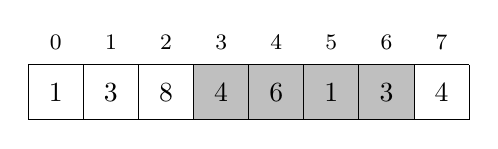
\begin{tikzpicture}[scale=0.7]
\fill[color=lightgray] (3,0) rectangle (7,1);
\draw (0,0) grid (8,1);

\node at (0.5,0.5) {$1$};
\node at (1.5,0.5) {$3$};
\node at (2.5,0.5) {$8$};
\node at (3.5,0.5) {$4$};
\node at (4.5,0.5) {$6$};
\node at (5.5,0.5) {$1$};
\node at (6.5,0.5) {$3$};
\node at (7.5,0.5) {$4$};

\footnotesize
\node at (0.5,1.4) {$0$};
\node at (1.5,1.4) {$1$};
\node at (2.5,1.4) {$2$};
\node at (3.5,1.4) {$3$};
\node at (4.5,1.4) {$4$};
\node at (5.5,1.4) {$5$};
\node at (6.5,1.4) {$6$};
\node at (7.5,1.4) {$7$};
\end{tikzpicture}
\end{center}
U ovom slučaju vrijedi $\texttt{sum}_q(3,6)=14$,
$\texttt{min}_q(3,6)=1$ i $\texttt{max}_q(3,6)=6$.

Jednostavan način obrade upita nad intervalima jest
petlja koja prolazi kroz sve vrijednosti niza u intervalu.
Na primjer, sljedeća se funkcija može
koristiti za obradu upita za sumu nad nizom:

\begin{lstlisting}
int sum(int a, int b) {
    int s = 0;
    for (int i = a; i <= b; i++) {
        s += array[i];
    }
    return s;
}
\end{lstlisting}

Ova funkcija radi u $O(n)$ vremenu,
gdje je $n$ veličina niza.
Stoga pomoću te funkcije možemo obraditi $q$ upita u $O(nq)$
vremenu.
Međutim, ako su i $n$ i $q$ veliki, ovaj je pristup
spor. Srećom, pokazuje se da postoje
načini za mnogo efikasniju obradu upita nad intervalima.

\section{Upiti nad statičkim nizom}

Najprije se usredotočimo na situaciju u kojoj je
niz \emph{statičan}, tj.
vrijednosti niza nikada se ne mijenjaju između upita.
U tom je slučaju dovoljno konstruirati
statičku strukturu podataka koja nam daje
odgovor na svaki mogući upit.

\subsubsection{Upiti za sumu}

\index{niz prefiksnih suma}

Upite za sumu nad statičkim nizom
možemo lako obraditi
konstruiranjem \key{niza prefiksnih suma}.
Svaka vrijednost u nizu prefiksnih suma jednaka je
sumi vrijednosti izvornog niza do te pozicije,
tj. vrijednost na poziciji $k$ jednaka je $\texttt{sum}_q(0,k)$.
Niz prefiksnih suma može se konstruirati u $O(n)$ vremenu.

Na primjer, promotrimo sljedeći niz:
\begin{center}
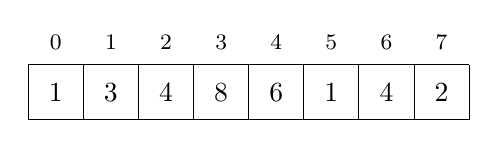
\begin{tikzpicture}[scale=0.7]
%\fill[color=lightgray] (3,0) rectangle (7,1);
\draw (0,0) grid (8,1);

\node at (0.5,0.5) {$1$};
\node at (1.5,0.5) {$3$};
\node at (2.5,0.5) {$4$};
\node at (3.5,0.5) {$8$};
\node at (4.5,0.5) {$6$};
\node at (5.5,0.5) {$1$};
\node at (6.5,0.5) {$4$};
\node at (7.5,0.5) {$2$};

\footnotesize
\node at (0.5,1.4) {$0$};
\node at (1.5,1.4) {$1$};
\node at (2.5,1.4) {$2$};
\node at (3.5,1.4) {$3$};
\node at (4.5,1.4) {$4$};
\node at (5.5,1.4) {$5$};
\node at (6.5,1.4) {$6$};
\node at (7.5,1.4) {$7$};
\end{tikzpicture}
\end{center}
Pripadni niz prefiksnih suma izgleda ovako:
\begin{center}
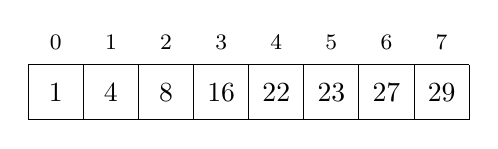
\begin{tikzpicture}[scale=0.7]
%\fill[color=lightgray] (3,0) rectangle (7,1);
\draw (0,0) grid (8,1);

\node at (0.5,0.5) {$1$};
\node at (1.5,0.5) {$4$};
\node at (2.5,0.5) {$8$};
\node at (3.5,0.5) {$16$};
\node at (4.5,0.5) {$22$};
\node at (5.5,0.5) {$23$};
\node at (6.5,0.5) {$27$};
\node at (7.5,0.5) {$29$};


\footnotesize
\node at (0.5,1.4) {$0$};
\node at (1.5,1.4) {$1$};
\node at (2.5,1.4) {$2$};
\node at (3.5,1.4) {$3$};
\node at (4.5,1.4) {$4$};
\node at (5.5,1.4) {$5$};
\node at (6.5,1.4) {$6$};
\node at (7.5,1.4) {$7$};
\end{tikzpicture}
\end{center}
Budući da niz prefiksnih suma sadrži sve vrijednosti
$\texttt{sum}_q(0,k)$,
svaku vrijednost
$\texttt{sum}_q(a,b)$ možemo izračunati u $O(1)$ vremenu ovako:
\[ \texttt{sum}_q(a,b) = \texttt{sum}_q(0,b) - \texttt{sum}_q(0,a-1)\]
Uz definiciju $\texttt{sum}_q(0,-1)=0$,
gornja formula vrijedi i kada je $a=0$.

Na primjer, promotrimo interval $[3,6]$:
\begin{center}
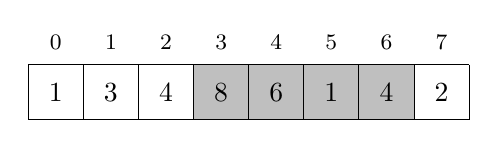
\begin{tikzpicture}[scale=0.7]
\fill[color=lightgray] (3,0) rectangle (7,1);
\draw (0,0) grid (8,1);

\node at (0.5,0.5) {$1$};
\node at (1.5,0.5) {$3$};
\node at (2.5,0.5) {$4$};
\node at (3.5,0.5) {$8$};
\node at (4.5,0.5) {$6$};
\node at (5.5,0.5) {$1$};
\node at (6.5,0.5) {$4$};
\node at (7.5,0.5) {$2$};

\footnotesize
\node at (0.5,1.4) {$0$};
\node at (1.5,1.4) {$1$};
\node at (2.5,1.4) {$2$};
\node at (3.5,1.4) {$3$};
\node at (4.5,1.4) {$4$};
\node at (5.5,1.4) {$5$};
\node at (6.5,1.4) {$6$};
\node at (7.5,1.4) {$7$};
\end{tikzpicture}
\end{center}
U ovom slučaju vrijedi $\texttt{sum}_q(3,6)=8+6+1+4=19$.
Ova se suma može izračunati iz
dviju vrijednosti niza prefiksnih suma:
\begin{center}
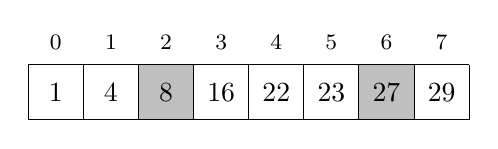
\begin{tikzpicture}[scale=0.7]
\fill[color=lightgray] (2,0) rectangle (3,1);
\fill[color=lightgray] (6,0) rectangle (7,1);
\draw (0,0) grid (8,1);

\node at (0.5,0.5) {$1$};
\node at (1.5,0.5) {$4$};
\node at (2.5,0.5) {$8$};
\node at (3.5,0.5) {$16$};
\node at (4.5,0.5) {$22$};
\node at (5.5,0.5) {$23$};
\node at (6.5,0.5) {$27$};
\node at (7.5,0.5) {$29$};

\footnotesize
\node at (0.5,1.4) {$0$};
\node at (1.5,1.4) {$1$};
\node at (2.5,1.4) {$2$};
\node at (3.5,1.4) {$3$};
\node at (4.5,1.4) {$4$};
\node at (5.5,1.4) {$5$};
\node at (6.5,1.4) {$6$};
\node at (7.5,1.4) {$7$};
\end{tikzpicture}
\end{center}
Dakle, $\texttt{sum}_q(3,6)=\texttt{sum}_q(0,6)-\texttt{sum}_q(0,2)=27-8=19$.

Ovu je ideju moguće poopćiti
i na više dimenzija.
Na primjer, možemo konstruirati dvodimenzionalni
niz prefiksnih suma pomoću kojega se može izračunati
suma bilo kojega pravokutnog podniza u $O(1)$ vremenu.
Svaka suma u takvom nizu odgovara
podnizu
koji počinje u gornjem lijevom kutu niza.

\begin{samepage}
Sljedeća slika ilustrira tu ideju:
\begin{center}
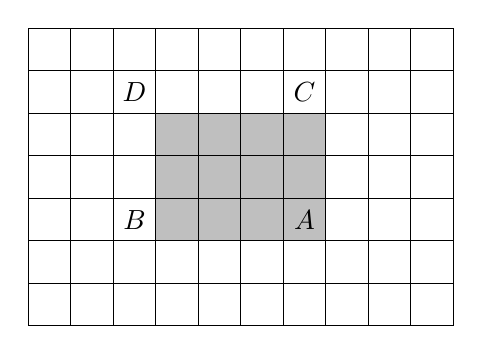
\begin{tikzpicture}[scale=0.54]
\draw[fill=lightgray] (3,2) rectangle (7,5);
\draw (0,0) grid (10,7);
\node[anchor=center] at (6.5, 2.5) {$A$};
\node[anchor=center] at (2.5, 2.5) {$B$};
\node[anchor=center] at (6.5, 5.5) {$C$};
\node[anchor=center] at (2.5, 5.5) {$D$};
\end{tikzpicture}
\end{center}
\end{samepage}

Suma sivog podniza može se izračunati
pomoću formule
\[S(A) - S(B) - S(C) + S(D),\]
gdje $S(X)$ označava sumu vrijednosti
u pravokutnom
podnizu od gornjega lijevog kuta
do pozicije od $X$.

\subsubsection{Upiti za minimum}

\index{rijetka tablica}

Upite za minimum teže je obraditi
nego upite za sumu.
Ipak, postoji prilično jednostavna 
metoda predobrade u $O(n \log n)$ vremenu
nakon koje možemo odgovoriti na svaki upit
za minimum u $O(1)$ vremenu\footnote{Ova tehnika
uvedena je u \cite{ben00} i ponekad se
naziva metodom \key{rijetke tablice}.
Postoje i sofisticiranije tehnike \cite{fis06} kod kojih
je vrijeme predobrade samo $O(n)$, ali takvi algoritmi
nisu potrebni u natjecateljskom programiranju.}.
Uočimo da se upiti za minimum i maksimum mogu
obraditi na sličan način,
pa se možemo usredotočiti na upite za minimum.

Ideja je unaprijed izračunati sve vrijednosti
$\textrm{min}_q(a,b)$ kod kojih je
$b-a+1$ (duljina intervala) potencija broja dva.
Na primjer, za niz

\begin{center}
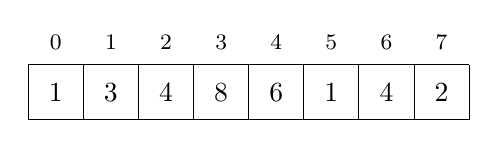
\begin{tikzpicture}[scale=0.7]
\draw (0,0) grid (8,1);

\node at (0.5,0.5) {$1$};
\node at (1.5,0.5) {$3$};
\node at (2.5,0.5) {$4$};
\node at (3.5,0.5) {$8$};
\node at (4.5,0.5) {$6$};
\node at (5.5,0.5) {$1$};
\node at (6.5,0.5) {$4$};
\node at (7.5,0.5) {$2$};

\footnotesize
\node at (0.5,1.4) {$0$};
\node at (1.5,1.4) {$1$};
\node at (2.5,1.4) {$2$};
\node at (3.5,1.4) {$3$};
\node at (4.5,1.4) {$4$};
\node at (5.5,1.4) {$5$};
\node at (6.5,1.4) {$6$};
\node at (7.5,1.4) {$7$};
\end{tikzpicture}
\end{center}
izračunavaju se sljedeće vrijednosti:

\begin{center}
\begin{tabular}{ccc}

\begin{tabular}{lll}
$a$ & $b$ & $\texttt{min}_q(a,b)$ \\
\hline
0 & 0 & 1 \\
1 & 1 & 3 \\
2 & 2 & 4 \\
3 & 3 & 8 \\
4 & 4 & 6 \\
5 & 5 & 1 \\
6 & 6 & 4 \\
7 & 7 & 2 \\
\end{tabular}

&

\begin{tabular}{lll}
$a$ & $b$ & $\texttt{min}_q(a,b)$ \\
\hline
0 & 1 & 1 \\
1 & 2 & 3 \\
2 & 3 & 4 \\
3 & 4 & 6 \\
4 & 5 & 1 \\
5 & 6 & 1 \\
6 & 7 & 2 \\
\\
\end{tabular}

&

\begin{tabular}{lll}
$a$ & $b$ & $\texttt{min}_q(a,b)$ \\
\hline
0 & 3 & 1 \\
1 & 4 & 3 \\
2 & 5 & 1 \\
3 & 6 & 1 \\
4 & 7 & 1 \\
0 & 7 & 1 \\
\\
\\
\end{tabular}

\end{tabular}
\end{center}

Broj unaprijed izračunatih vrijednosti je $O(n \log n)$,
jer postoji $O(\log n)$ duljina intervala
koje su potencije broja dva.
Vrijednosti se mogu efikasno izračunati
pomoću rekurzivne formule
\[\texttt{min}_q(a,b) = \min(\texttt{min}_q(a,a+w-1),\texttt{min}_q(a+w,b)),\]
gdje je $b-a+1$ potencija broja dva i $w=(b-a+1)/2$.
Izračunavanje svih tih vrijednosti traži $O(n \log n)$ vremena.

Nakon toga svaka se vrijednost $\texttt{min}_q(a,b)$ može izračunati
u $O(1)$ vremenu kao minimum dviju unaprijed izračunatih vrijednosti.
Neka je $k$ najveća potencija broja dva koja ne prelazi $b-a+1$.
Vrijednost $\texttt{min}_q(a,b)$ možemo izračunati pomoću formule
\[\texttt{min}_q(a,b) = \min(\texttt{min}_q(a,a+k-1),\texttt{min}_q(b-k+1,b)).\]
U gornjoj je formuli interval $[a,b]$ prikazan
kao unija intervala $[a,a+k-1]$ i $[b-k+1,b]$, oba duljine $k$.

Kao primjer, promotrimo interval $[1,6]$:
\begin{center}
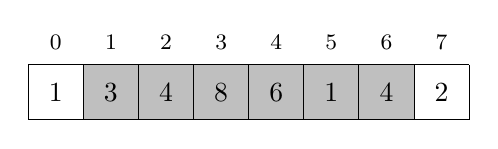
\begin{tikzpicture}[scale=0.7]
\fill[color=lightgray] (1,0) rectangle (7,1);
\draw (0,0) grid (8,1);

\node at (0.5,0.5) {$1$};
\node at (1.5,0.5) {$3$};
\node at (2.5,0.5) {$4$};
\node at (3.5,0.5) {$8$};
\node at (4.5,0.5) {$6$};
\node at (5.5,0.5) {$1$};
\node at (6.5,0.5) {$4$};
\node at (7.5,0.5) {$2$};

\footnotesize
\node at (0.5,1.4) {$0$};
\node at (1.5,1.4) {$1$};
\node at (2.5,1.4) {$2$};
\node at (3.5,1.4) {$3$};
\node at (4.5,1.4) {$4$};
\node at (5.5,1.4) {$5$};
\node at (6.5,1.4) {$6$};
\node at (7.5,1.4) {$7$};
\end{tikzpicture}
\end{center}
Duljina intervala je 6,
a najveća potencija broja dva koja
ne prelazi 6 jest 4.
Stoga je interval $[1,6]$
unija intervala $[1,4]$ i $[3,6]$:
\begin{center}
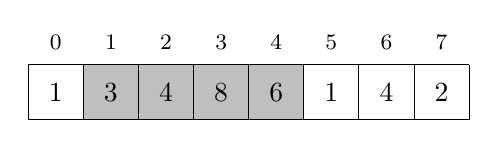
\begin{tikzpicture}[scale=0.7]
\fill[color=lightgray] (1,0) rectangle (5,1);
\draw (0,0) grid (8,1);

\node at (0.5,0.5) {$1$};
\node at (1.5,0.5) {$3$};
\node at (2.5,0.5) {$4$};
\node at (3.5,0.5) {$8$};
\node at (4.5,0.5) {$6$};
\node at (5.5,0.5) {$1$};
\node at (6.5,0.5) {$4$};
\node at (7.5,0.5) {$2$};

\footnotesize
\node at (0.5,1.4) {$0$};
\node at (1.5,1.4) {$1$};
\node at (2.5,1.4) {$2$};
\node at (3.5,1.4) {$3$};
\node at (4.5,1.4) {$4$};
\node at (5.5,1.4) {$5$};
\node at (6.5,1.4) {$6$};
\node at (7.5,1.4) {$7$};
\end{tikzpicture}
\end{center}
\begin{center}
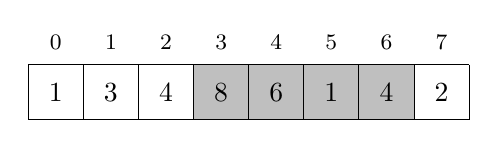
\begin{tikzpicture}[scale=0.7]
\fill[color=lightgray] (3,0) rectangle (7,1);
\draw (0,0) grid (8,1);

\node at (0.5,0.5) {$1$};
\node at (1.5,0.5) {$3$};
\node at (2.5,0.5) {$4$};
\node at (3.5,0.5) {$8$};
\node at (4.5,0.5) {$6$};
\node at (5.5,0.5) {$1$};
\node at (6.5,0.5) {$4$};
\node at (7.5,0.5) {$2$};


\footnotesize
\node at (0.5,1.4) {$0$};
\node at (1.5,1.4) {$1$};
\node at (2.5,1.4) {$2$};
\node at (3.5,1.4) {$3$};
\node at (4.5,1.4) {$4$};
\node at (5.5,1.4) {$5$};
\node at (6.5,1.4) {$6$};
\node at (7.5,1.4) {$7$};
\end{tikzpicture}
\end{center}
Budući da je $\texttt{min}_q(1,4)=3$ i $\texttt{min}_q(3,6)=1$,
zaključujemo da je $\texttt{min}_q(1,6)=1$.

\section{Binarno indeksirano stablo}

\index{binarno indeksirano stablo}
\index{Fenwickovo stablo}

\key{Binarno indeksirano stablo} ili \key{Fenwickovo stablo}\footnote{Strukturu
binarno indeksiranog stabla predstavio je P. M. Fenwick 1994. godine \cite{fen94}.}
može se promatrati kao dinamička inačica niza prefiksnih suma.
Podržava dvije operacije nad nizom u $O(\log n)$ vremenu:
obradu upita za sumu nad intervalom i ažuriranje vrijednosti.

Prednost binarno indeksiranog stabla jest
to što nam omogućuje efikasno ažuriranje
vrijednosti niza između upita za sumu.
To ne bi bilo moguće s nizom prefiksnih suma,
jer bi nakon svakog ažuriranja bilo potrebno ponovno izgraditi
cijeli niz prefiksnih suma u $O(n)$ vremenu.

\subsubsection{Struktura}

Iako se struktura zove binarno indeksirano \emph{stablo},
obično se prikazuje kao niz.
U ovom odjeljku pretpostavljamo da su svi nizovi indeksirani od jedinice,
jer to olakšava implementaciju.

Neka $p(k)$ označava najveću potenciju broja dva koja
dijeli $k$.
Binarno indeksirano stablo pohranjujemo kao niz \texttt{tree}
tako da vrijedi
\[ \texttt{tree}[k] = \texttt{sum}_q(k-p(k)+1,k),\]
tj. svaka pozicija $k$ sadrži sumu vrijednosti
u intervalu izvornog niza čija je duljina $p(k)$
i koji završava na poziciji $k$.
Na primjer, budući da je $p(6)=2$, $\texttt{tree}[6]$
sadrži vrijednost $\texttt{sum}_q(5,6)$.

Na primjer, promotrimo sljedeći niz:
\begin{center}
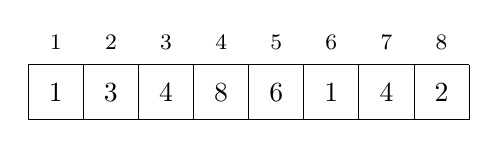
\begin{tikzpicture}[scale=0.7]
\draw (0,0) grid (8,1);

\node at (0.5,0.5) {$1$};
\node at (1.5,0.5) {$3$};
\node at (2.5,0.5) {$4$};
\node at (3.5,0.5) {$8$};
\node at (4.5,0.5) {$6$};
\node at (5.5,0.5) {$1$};
\node at (6.5,0.5) {$4$};
\node at (7.5,0.5) {$2$};

\footnotesize
\node at (0.5,1.4) {$1$};
\node at (1.5,1.4) {$2$};
\node at (2.5,1.4) {$3$};
\node at (3.5,1.4) {$4$};
\node at (4.5,1.4) {$5$};
\node at (5.5,1.4) {$6$};
\node at (6.5,1.4) {$7$};
\node at (7.5,1.4) {$8$};
\end{tikzpicture}
\end{center}

Pripadno binarno indeksirano stablo izgleda ovako:
\begin{center}
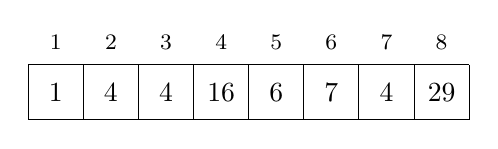
\begin{tikzpicture}[scale=0.7]
\draw (0,0) grid (8,1);

\node at (0.5,0.5) {$1$};
\node at (1.5,0.5) {$4$};
\node at (2.5,0.5) {$4$};
\node at (3.5,0.5) {$16$};
\node at (4.5,0.5) {$6$};
\node at (5.5,0.5) {$7$};
\node at (6.5,0.5) {$4$};
\node at (7.5,0.5) {$29$};

\footnotesize
\node at (0.5,1.4) {$1$};
\node at (1.5,1.4) {$2$};
\node at (2.5,1.4) {$3$};
\node at (3.5,1.4) {$4$};
\node at (4.5,1.4) {$5$};
\node at (5.5,1.4) {$6$};
\node at (6.5,1.4) {$7$};
\node at (7.5,1.4) {$8$};
\end{tikzpicture}
\end{center}

Sljedeća slika jasnije pokazuje
kako svaka vrijednost u binarno indeksiranom stablu
odgovara jednom intervalu izvornog niza:

\begin{center}
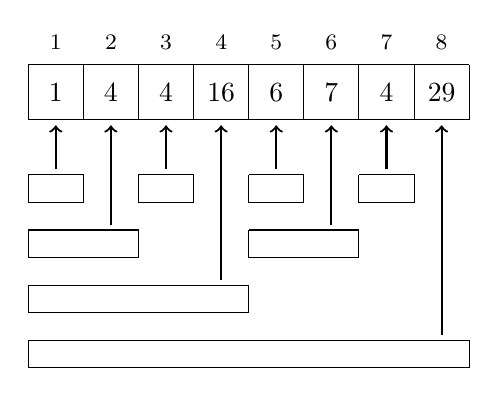
\begin{tikzpicture}[scale=0.7]
\draw (0,0) grid (8,1);

\node at (0.5,0.5) {$1$};
\node at (1.5,0.5) {$4$};
\node at (2.5,0.5) {$4$};
\node at (3.5,0.5) {$16$};
\node at (4.5,0.5) {$6$};
\node at (5.5,0.5) {$7$};
\node at (6.5,0.5) {$4$};
\node at (7.5,0.5) {$29$};

\footnotesize
\node at (0.5,1.4) {$1$};
\node at (1.5,1.4) {$2$};
\node at (2.5,1.4) {$3$};
\node at (3.5,1.4) {$4$};
\node at (4.5,1.4) {$5$};
\node at (5.5,1.4) {$6$};
\node at (6.5,1.4) {$7$};
\node at (7.5,1.4) {$8$};

\draw[->,thick] (0.5,-0.9) -- (0.5,-0.1);
\draw[->,thick] (2.5,-0.9) -- (2.5,-0.1);
\draw[->,thick] (4.5,-0.9) -- (4.5,-0.1);
\draw[->,thick] (6.5,-0.9) -- (6.5,-0.1);
\draw[->,thick] (1.5,-1.9) -- (1.5,-0.1);
\draw[->,thick] (5.5,-1.9) -- (5.5,-0.1);
\draw[->,thick] (3.5,-2.9) -- (3.5,-0.1);
\draw[->,thick] (7.5,-3.9) -- (7.5,-0.1);

\draw (0,-1) -- (1,-1) -- (1,-1.5) -- (0,-1.5) -- (0,-1);
\draw (2,-1) -- (3,-1) -- (3,-1.5) -- (2,-1.5) -- (2,-1);
\draw (4,-1) -- (5,-1) -- (5,-1.5) -- (4,-1.5) -- (4,-1);
\draw (6,-1) -- (7,-1) -- (7,-1.5) -- (6,-1.5) -- (6,-1);
\draw (0,-2) -- (2,-2) -- (2,-2.5) -- (0,-2.5) -- (0,-2);
\draw (4,-2) -- (6,-2) -- (6,-2.5) -- (4,-2.5) -- (4,-2);
\draw (0,-3) -- (4,-3) -- (4,-3.5) -- (0,-3.5) -- (0,-3);
\draw (0,-4) -- (8,-4) -- (8,-4.5) -- (0,-4.5) -- (0,-4);
\end{tikzpicture}
\end{center}

Pomoću binarno indeksiranog stabla
svaka se vrijednost $\texttt{sum}_q(1,k)$
može izračunati u $O(\log n)$ vremenu,
jer se interval $[1,k]$ uvijek može podijeliti na
$O(\log n)$ intervala čije su sume pohranjene u stablu.

Na primjer, interval $[1,7]$ sastoji se od
sljedećih intervala:
\begin{center}
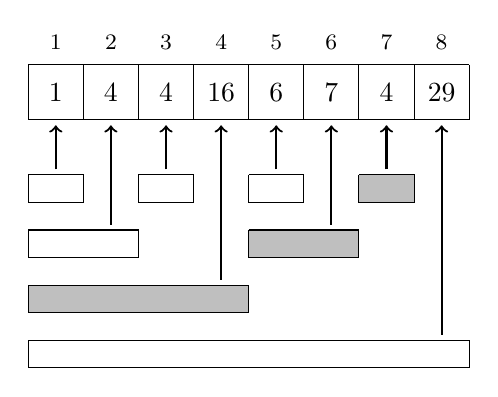
\begin{tikzpicture}[scale=0.7]
\draw (0,0) grid (8,1);

\node at (0.5,0.5) {$1$};
\node at (1.5,0.5) {$4$};
\node at (2.5,0.5) {$4$};
\node at (3.5,0.5) {$16$};
\node at (4.5,0.5) {$6$};
\node at (5.5,0.5) {$7$};
\node at (6.5,0.5) {$4$};
\node at (7.5,0.5) {$29$};

\footnotesize
\node at (0.5,1.4) {$1$};
\node at (1.5,1.4) {$2$};
\node at (2.5,1.4) {$3$};
\node at (3.5,1.4) {$4$};
\node at (4.5,1.4) {$5$};
\node at (5.5,1.4) {$6$};
\node at (6.5,1.4) {$7$};
\node at (7.5,1.4) {$8$};

\draw[->,thick] (0.5,-0.9) -- (0.5,-0.1);
\draw[->,thick] (2.5,-0.9) -- (2.5,-0.1);
\draw[->,thick] (4.5,-0.9) -- (4.5,-0.1);
\draw[->,thick] (6.5,-0.9) -- (6.5,-0.1);
\draw[->,thick] (1.5,-1.9) -- (1.5,-0.1);
\draw[->,thick] (5.5,-1.9) -- (5.5,-0.1);
\draw[->,thick] (3.5,-2.9) -- (3.5,-0.1);
\draw[->,thick] (7.5,-3.9) -- (7.5,-0.1);

\draw (0,-1) -- (1,-1) -- (1,-1.5) -- (0,-1.5) -- (0,-1);
\draw (2,-1) -- (3,-1) -- (3,-1.5) -- (2,-1.5) -- (2,-1);
\draw (4,-1) -- (5,-1) -- (5,-1.5) -- (4,-1.5) -- (4,-1);
\draw[fill=lightgray] (6,-1) -- (7,-1) -- (7,-1.5) -- (6,-1.5) -- (6,-1);
\draw (0,-2) -- (2,-2) -- (2,-2.5) -- (0,-2.5) -- (0,-2);
\draw[fill=lightgray] (4,-2) -- (6,-2) -- (6,-2.5) -- (4,-2.5) -- (4,-2);
\draw[fill=lightgray] (0,-3) -- (4,-3) -- (4,-3.5) -- (0,-3.5) -- (0,-3);
\draw (0,-4) -- (8,-4) -- (8,-4.5) -- (0,-4.5) -- (0,-4);
\end{tikzpicture}
\end{center}
Pripadnu sumu stoga možemo izračunati ovako:
\[\texttt{sum}_q(1,7)=\texttt{sum}_q(1,4)+\texttt{sum}_q(5,6)+\texttt{sum}_q(7,7)=16+7+4=27\]

Za izračun vrijednosti $\texttt{sum}_q(a,b)$ gdje je $a>1$
možemo upotrijebiti isti trik koji smo koristili kod nizova prefiksnih suma:
\[ \texttt{sum}_q(a,b) = \texttt{sum}_q(1,b) - \texttt{sum}_q(1,a-1).\]
Budući da i $\texttt{sum}_q(1,b)$
i $\texttt{sum}_q(1,a-1)$ možemo izračunati u $O(\log n)$ vremenu,
ukupna je vremenska složenost $O(\log n)$.

Nadalje, nakon ažuriranja vrijednosti u izvornom nizu
treba ažurirati nekoliko vrijednosti
u binarno indeksiranom stablu.
Na primjer, ako se promijeni vrijednost na poziciji 3,
mijenjaju se sume sljedećih intervala:
\begin{center}
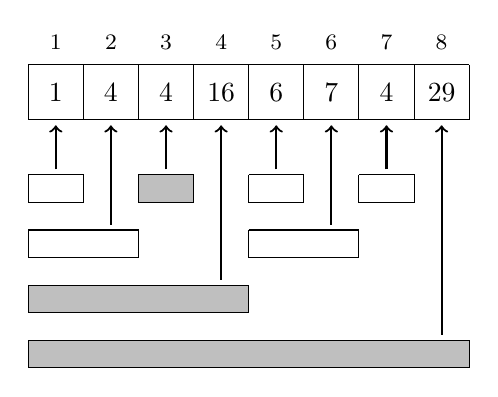
\begin{tikzpicture}[scale=0.7]
\draw (0,0) grid (8,1);

\node at (0.5,0.5) {$1$};
\node at (1.5,0.5) {$4$};
\node at (2.5,0.5) {$4$};
\node at (3.5,0.5) {$16$};
\node at (4.5,0.5) {$6$};
\node at (5.5,0.5) {$7$};
\node at (6.5,0.5) {$4$};
\node at (7.5,0.5) {$29$};

\footnotesize
\node at (0.5,1.4) {$1$};
\node at (1.5,1.4) {$2$};
\node at (2.5,1.4) {$3$};
\node at (3.5,1.4) {$4$};
\node at (4.5,1.4) {$5$};
\node at (5.5,1.4) {$6$};
\node at (6.5,1.4) {$7$};
\node at (7.5,1.4) {$8$};

\draw[->,thick] (0.5,-0.9) -- (0.5,-0.1);
\draw[->,thick] (2.5,-0.9) -- (2.5,-0.1);
\draw[->,thick] (4.5,-0.9) -- (4.5,-0.1);
\draw[->,thick] (6.5,-0.9) -- (6.5,-0.1);
\draw[->,thick] (1.5,-1.9) -- (1.5,-0.1);
\draw[->,thick] (5.5,-1.9) -- (5.5,-0.1);
\draw[->,thick] (3.5,-2.9) -- (3.5,-0.1);
\draw[->,thick] (7.5,-3.9) -- (7.5,-0.1);

\draw (0,-1) -- (1,-1) -- (1,-1.5) -- (0,-1.5) -- (0,-1);
\draw[fill=lightgray] (2,-1) -- (3,-1) -- (3,-1.5) -- (2,-1.5) -- (2,-1);
\draw (4,-1) -- (5,-1) -- (5,-1.5) -- (4,-1.5) -- (4,-1);
\draw (6,-1) -- (7,-1) -- (7,-1.5) -- (6,-1.5) -- (6,-1);
\draw (0,-2) -- (2,-2) -- (2,-2.5) -- (0,-2.5) -- (0,-2);
\draw (4,-2) -- (6,-2) -- (6,-2.5) -- (4,-2.5) -- (4,-2);
\draw[fill=lightgray] (0,-3) -- (4,-3) -- (4,-3.5) -- (0,-3.5) -- (0,-3);
\draw[fill=lightgray] (0,-4) -- (8,-4) -- (8,-4.5) -- (0,-4.5) -- (0,-4);
\end{tikzpicture}
\end{center}

Budući da svaki element niza pripada $O(\log n)$
intervala u binarno indeksiranom stablu,
dovoljno je ažurirati $O(\log n)$ vrijednosti u stablu.

\subsubsection{Implementacija}

Operacije binarno indeksiranog stabla mogu se
efikasno implementirati pomoću bitovnih operacija.
Ključna je činjenica da svaku vrijednost $p(k)$
možemo izračunati pomoću formule
\[p(k) = k \& -k.\]

Sljedeća funkcija računa vrijednost $\texttt{sum}_q(1,k)$:
\begin{lstlisting}
int sum(int k) {
    int s = 0;
    while (k >= 1) {
        s += tree[k];
        k -= k&-k;
    }
    return s;
}
\end{lstlisting}

Sljedeća funkcija povećava
vrijednost niza na poziciji $k$ za $x$
($x$ može biti pozitivan ili negativan):
\begin{lstlisting}
void add(int k, int x) {
    while (k <= n) {
        tree[k] += x;
        k += k&-k;
    }
}
\end{lstlisting}

Vremenska složenost obiju funkcija je
$O(\log n)$, jer funkcije pristupaju $O(\log n)$
vrijednostima u binarno indeksiranom stablu, a svaki pomak
na sljedeću poziciju traži $O(1)$ vremena.

\section{Segmentno stablo}

\index{segmentno stablo}

\key{Segmentno stablo}\footnote{Implementacija odozdo prema gore u ovom poglavlju odgovara
onoj u \cite{sta06}. Slične su se strukture koristile
krajem 1970-ih za rješavanje geometrijskih zadataka \cite{ben80}.} je struktura podataka
koja podržava dvije operacije:
obradu upita nad intervalom i
ažuriranje vrijednosti niza.
Segmentna stabla mogu podržati
upite za sumu, upite za minimum i maksimum te mnoge druge
upite tako da obje operacije rade u $O(\log n)$ vremenu.

U usporedbi s binarno indeksiranim stablom,
prednost je segmentnog stabla to što je
općenitija struktura podataka.
Dok binarno indeksirana stabla podržavaju samo
upite za sumu\footnote{Zapravo, pomoću \emph{dvaju} binarno
indeksiranih stabala moguće je podržati upite za minimum \cite{dim15},
ali to je složenije od korištenja segmentnog stabla.},
segmentna stabla podržavaju i druge upite.
S druge strane, segmentno stablo traži više
memorije i nešto ga je teže implementirati.

\subsubsection{Struktura}

Segmentno stablo je binarno stablo
u kojem čvorovi na najnižoj razini stabla
odgovaraju elementima niza,
a ostali čvorovi
sadrže informacije potrebne za obradu upita nad intervalima.

U ovom odjeljku pretpostavljamo da je veličina
niza potencija broja dva i da se koristi
indeksiranje od nule, jer je za takav niz
zgodno izgraditi segmentno stablo.
Ako veličina niza nije potencija broja dva,
uvijek mu možemo dodati dodatne elemente.

Najprije ćemo razmotriti segmentna stabla koja podržavaju upite za sumu.
Kao primjer, promotrimo sljedeći niz:
\begin{center}
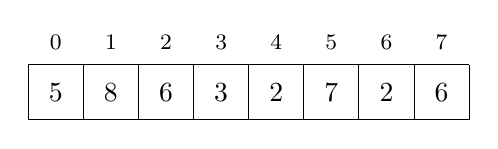
\begin{tikzpicture}[scale=0.7]
\draw (0,0) grid (8,1);

\node at (0.5,0.5) {$5$};
\node at (1.5,0.5) {$8$};
\node at (2.5,0.5) {$6$};
\node at (3.5,0.5) {$3$};
\node at (4.5,0.5) {$2$};
\node at (5.5,0.5) {$7$};
\node at (6.5,0.5) {$2$};
\node at (7.5,0.5) {$6$};

\footnotesize
\node at (0.5,1.4) {$0$};
\node at (1.5,1.4) {$1$};
\node at (2.5,1.4) {$2$};
\node at (3.5,1.4) {$3$};
\node at (4.5,1.4) {$4$};
\node at (5.5,1.4) {$5$};
\node at (6.5,1.4) {$6$};
\node at (7.5,1.4) {$7$};
\end{tikzpicture}
\end{center}
Pripadno segmentno stablo izgleda ovako:
\begin{center}
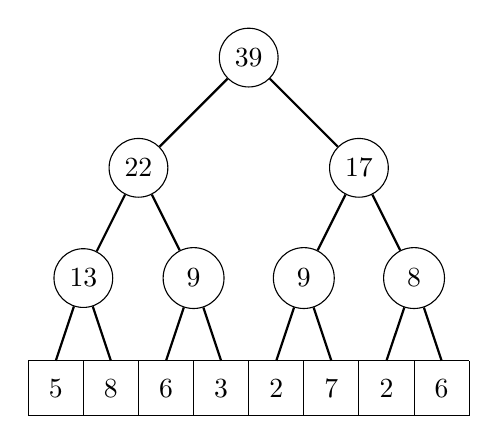
\begin{tikzpicture}[scale=0.7]
\draw (0,0) grid (8,1);

\node[anchor=center] at (0.5, 0.5) {5};
\node[anchor=center] at (1.5, 0.5) {8};
\node[anchor=center] at (2.5, 0.5) {6};
\node[anchor=center] at (3.5, 0.5) {3};
\node[anchor=center] at (4.5, 0.5) {2};
\node[anchor=center] at (5.5, 0.5) {7};
\node[anchor=center] at (6.5, 0.5) {2};
\node[anchor=center] at (7.5, 0.5) {6};

\node[draw, circle] (a) at (1,2.5) {13};
\path[draw,thick,-] (a) -- (0.5,1);
\path[draw,thick,-] (a) -- (1.5,1);
\node[draw, circle,minimum size=22pt] (b) at (3,2.5) {9};
\path[draw,thick,-] (b) -- (2.5,1);
\path[draw,thick,-] (b) -- (3.5,1);
\node[draw, circle,minimum size=22pt] (c) at (5,2.5) {9};
\path[draw,thick,-] (c) -- (4.5,1);
\path[draw,thick,-] (c) -- (5.5,1);
\node[draw, circle,minimum size=22pt] (d) at (7,2.5) {8};
\path[draw,thick,-] (d) -- (6.5,1);
\path[draw,thick,-] (d) -- (7.5,1);

\node[draw, circle] (i) at (2,4.5) {22};
\path[draw,thick,-] (i) -- (a);
\path[draw,thick,-] (i) -- (b);
\node[draw, circle] (j) at (6,4.5) {17};
\path[draw,thick,-] (j) -- (c);
\path[draw,thick,-] (j) -- (d);

\node[draw, circle] (m) at (4,6.5) {39};
\path[draw,thick,-] (m) -- (i);
\path[draw,thick,-] (m) -- (j);
\end{tikzpicture}
\end{center}

Svaki unutarnji čvor stabla
odgovara intervalu niza
čija je veličina potencija broja dva.
U gornjem stablu vrijednost svakoga unutarnjeg
čvora jednaka je sumi pripadnih vrijednosti niza,
a može se izračunati kao suma
vrijednosti njegova lijevog i desnog djeteta.

Pokazuje se da se svaki interval $[a,b]$
može podijeliti na $O(\log n)$ intervala
čije su vrijednosti pohranjene u čvorovima stabla.
Na primjer, promotrimo interval [2,7]:
\begin{center}
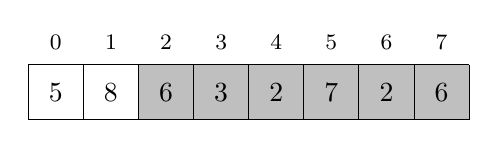
\begin{tikzpicture}[scale=0.7]
\fill[color=gray!50] (2,0) rectangle (8,1);
\draw (0,0) grid (8,1);

\node[anchor=center] at (0.5, 0.5) {5};
\node[anchor=center] at (1.5, 0.5) {8};
\node[anchor=center] at (2.5, 0.5) {6};
\node[anchor=center] at (3.5, 0.5) {3};
\node[anchor=center] at (4.5, 0.5) {2};
\node[anchor=center] at (5.5, 0.5) {7};
\node[anchor=center] at (6.5, 0.5) {2};
\node[anchor=center] at (7.5, 0.5) {6};

\footnotesize
\node at (0.5,1.4) {$0$};
\node at (1.5,1.4) {$1$};
\node at (2.5,1.4) {$2$};
\node at (3.5,1.4) {$3$};
\node at (4.5,1.4) {$4$};
\node at (5.5,1.4) {$5$};
\node at (6.5,1.4) {$6$};
\node at (7.5,1.4) {$7$};
\end{tikzpicture}
\end{center}
Ovdje je $\texttt{sum}_q(2,7)=6+3+2+7+2+6=26$.
U ovom slučaju intervalu odgovaraju
sljedeća dva čvora stabla:
\begin{center}
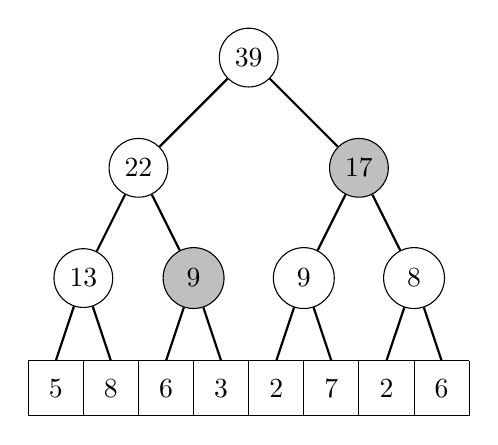
\begin{tikzpicture}[scale=0.7]
\draw (0,0) grid (8,1);

\node[anchor=center] at (0.5, 0.5) {5};
\node[anchor=center] at (1.5, 0.5) {8};
\node[anchor=center] at (2.5, 0.5) {6};
\node[anchor=center] at (3.5, 0.5) {3};
\node[anchor=center] at (4.5, 0.5) {2};
\node[anchor=center] at (5.5, 0.5) {7};
\node[anchor=center] at (6.5, 0.5) {2};
\node[anchor=center] at (7.5, 0.5) {6};

\node[draw, circle] (a) at (1,2.5) {13};
\path[draw,thick,-] (a) -- (0.5,1);
\path[draw,thick,-] (a) -- (1.5,1);
\node[draw, circle,fill=gray!50,minimum size=22pt] (b) at (3,2.5) {9};
\path[draw,thick,-] (b) -- (2.5,1);
\path[draw,thick,-] (b) -- (3.5,1);
\node[draw, circle,minimum size=22pt] (c) at (5,2.5) {9};
\path[draw,thick,-] (c) -- (4.5,1);
\path[draw,thick,-] (c) -- (5.5,1);
\node[draw, circle,minimum size=22pt] (d) at (7,2.5) {8};
\path[draw,thick,-] (d) -- (6.5,1);
\path[draw,thick,-] (d) -- (7.5,1);

\node[draw, circle] (i) at (2,4.5) {22};
\path[draw,thick,-] (i) -- (a);
\path[draw,thick,-] (i) -- (b);
\node[draw, circle,fill=gray!50] (j) at (6,4.5) {17};
\path[draw,thick,-] (j) -- (c);
\path[draw,thick,-] (j) -- (d);

\node[draw, circle] (m) at (4,6.5) {39};
\path[draw,thick,-] (m) -- (i);
\path[draw,thick,-] (m) -- (j);
\end{tikzpicture}
\end{center}
Dakle, sumu možemo izračunati i kao $9+17=26$.

Kada se suma računa pomoću čvorova
što više u stablu,
potrebna su najviše dva čvora
na svakoj razini stabla.
Stoga je ukupan broj čvorova
$O(\log n)$.

Nakon ažuriranja niza
trebamo ažurirati sve čvorove
čija vrijednost ovisi o ažuriranoj vrijednosti.
To se može učiniti prolaskom putem
od ažuriranog elementa niza do najvišeg čvora
uz ažuriranje čvorova na tom putu.

Sljedeća slika pokazuje koji se čvorovi stabla
mijenjaju ako se promijeni vrijednost niza 7:

\begin{center}
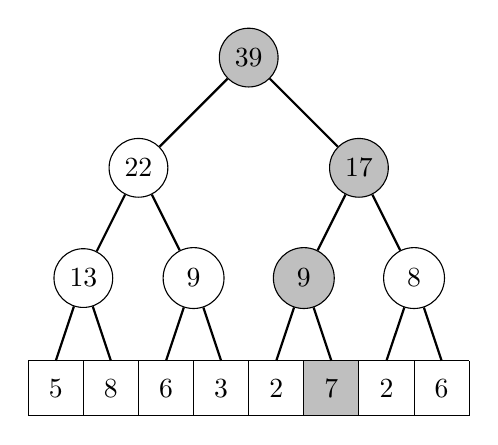
\begin{tikzpicture}[scale=0.7]
\fill[color=gray!50] (5,0) rectangle (6,1);
\draw (0,0) grid (8,1);

\node[anchor=center] at (0.5, 0.5) {5};
\node[anchor=center] at (1.5, 0.5) {8};
\node[anchor=center] at (2.5, 0.5) {6};
\node[anchor=center] at (3.5, 0.5) {3};
\node[anchor=center] at (4.5, 0.5) {2};
\node[anchor=center] at (5.5, 0.5) {7};
\node[anchor=center] at (6.5, 0.5) {2};
\node[anchor=center] at (7.5, 0.5) {6};

\node[draw, circle] (a) at (1,2.5) {13};
\path[draw,thick,-] (a) -- (0.5,1);
\path[draw,thick,-] (a) -- (1.5,1);
\node[draw, circle,minimum size=22pt] (b) at (3,2.5) {9};
\path[draw,thick,-] (b) -- (2.5,1);
\path[draw,thick,-] (b) -- (3.5,1);
\node[draw, circle,minimum size=22pt,fill=gray!50] (c) at (5,2.5) {9};
\path[draw,thick,-] (c) -- (4.5,1);
\path[draw,thick,-] (c) -- (5.5,1);
\node[draw, circle,minimum size=22pt] (d) at (7,2.5) {8};
\path[draw,thick,-] (d) -- (6.5,1);
\path[draw,thick,-] (d) -- (7.5,1);

\node[draw, circle] (i) at (2,4.5) {22};
\path[draw,thick,-] (i) -- (a);
\path[draw,thick,-] (i) -- (b);
\node[draw, circle,fill=gray!50] (j) at (6,4.5) {17};
\path[draw,thick,-] (j) -- (c);
\path[draw,thick,-] (j) -- (d);

\node[draw, circle,fill=gray!50] (m) at (4,6.5) {39};
\path[draw,thick,-] (m) -- (i);
\path[draw,thick,-] (m) -- (j);
\end{tikzpicture}
\end{center}

Put od dna prema vrhu
uvijek se sastoji od $O(\log n)$ čvorova,
pa svako ažuriranje mijenja $O(\log n)$ čvorova u stablu.

\subsubsection{Implementacija}

Segmentno stablo pohranjujemo kao niz
od $2n$ elemenata, gdje je $n$ veličina
izvornog niza i potencija broja dva.
Čvorovi stabla pohranjuju se odozgo prema dolje:
$\texttt{tree}[1]$ je najviši čvor,
$\texttt{tree}[2]$ i $\texttt{tree}[3]$
njegova su djeca, i tako dalje.
Naposljetku, vrijednosti od $\texttt{tree}[n]$
do $\texttt{tree}[2n-1]$ odgovaraju
vrijednostima izvornog niza
na najnižoj razini stabla.

Na primjer, segmentno stablo
\begin{center}
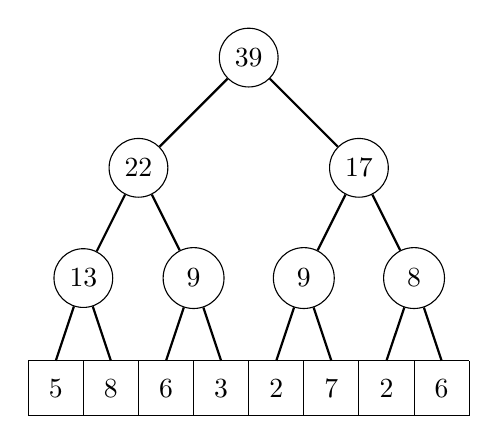
\begin{tikzpicture}[scale=0.7]
\draw (0,0) grid (8,1);

\node[anchor=center] at (0.5, 0.5) {5};
\node[anchor=center] at (1.5, 0.5) {8};
\node[anchor=center] at (2.5, 0.5) {6};
\node[anchor=center] at (3.5, 0.5) {3};
\node[anchor=center] at (4.5, 0.5) {2};
\node[anchor=center] at (5.5, 0.5) {7};
\node[anchor=center] at (6.5, 0.5) {2};
\node[anchor=center] at (7.5, 0.5) {6};

\node[draw, circle] (a) at (1,2.5) {13};
\path[draw,thick,-] (a) -- (0.5,1);
\path[draw,thick,-] (a) -- (1.5,1);
\node[draw, circle,minimum size=22pt] (b) at (3,2.5) {9};
\path[draw,thick,-] (b) -- (2.5,1);
\path[draw,thick,-] (b) -- (3.5,1);
\node[draw, circle,minimum size=22pt] (c) at (5,2.5) {9};
\path[draw,thick,-] (c) -- (4.5,1);
\path[draw,thick,-] (c) -- (5.5,1);
\node[draw, circle,minimum size=22pt] (d) at (7,2.5) {8};
\path[draw,thick,-] (d) -- (6.5,1);
\path[draw,thick,-] (d) -- (7.5,1);

\node[draw, circle] (i) at (2,4.5) {22};
\path[draw,thick,-] (i) -- (a);
\path[draw,thick,-] (i) -- (b);
\node[draw, circle] (j) at (6,4.5) {17};
\path[draw,thick,-] (j) -- (c);
\path[draw,thick,-] (j) -- (d);

\node[draw, circle] (m) at (4,6.5) {39};
\path[draw,thick,-] (m) -- (i);
\path[draw,thick,-] (m) -- (j);
\end{tikzpicture}
\end{center}
pohranjuje se ovako:
\begin{center}
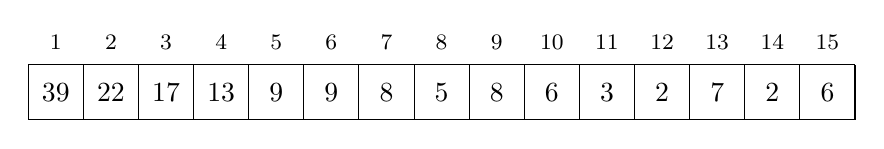
\begin{tikzpicture}[scale=0.7]
\draw (0,0) grid (15,1);

\node at (0.5,0.5) {$39$};
\node at (1.5,0.5) {$22$};
\node at (2.5,0.5) {$17$};
\node at (3.5,0.5) {$13$};
\node at (4.5,0.5) {$9$};
\node at (5.5,0.5) {$9$};
\node at (6.5,0.5) {$8$};
\node at (7.5,0.5) {$5$};
\node at (8.5,0.5) {$8$};
\node at (9.5,0.5) {$6$};
\node at (10.5,0.5) {$3$};
\node at (11.5,0.5) {$2$};
\node at (12.5,0.5) {$7$};
\node at (13.5,0.5) {$2$};
\node at (14.5,0.5) {$6$};

\footnotesize
\node at (0.5,1.4) {$1$};
\node at (1.5,1.4) {$2$};
\node at (2.5,1.4) {$3$};
\node at (3.5,1.4) {$4$};
\node at (4.5,1.4) {$5$};
\node at (5.5,1.4) {$6$};
\node at (6.5,1.4) {$7$};
\node at (7.5,1.4) {$8$};
\node at (8.5,1.4) {$9$};
\node at (9.5,1.4) {$10$};
\node at (10.5,1.4) {$11$};
\node at (11.5,1.4) {$12$};
\node at (12.5,1.4) {$13$};
\node at (13.5,1.4) {$14$};
\node at (14.5,1.4) {$15$};
\end{tikzpicture}
\end{center}
Uz ovaj prikaz
roditelj čvora $\texttt{tree}[k]$
jest $\texttt{tree}[\lfloor k/2 \rfloor]$,
a njegova su djeca $\texttt{tree}[2k]$
i $\texttt{tree}[2k+1]$.
Uočimo da to znači da je pozicija čvora
parna ako je on lijevo dijete, a neparna ako je desno dijete.

Sljedeća funkcija
računa vrijednost $\texttt{sum}_q(a,b)$:
\begin{lstlisting}
int sum(int a, int b) {
    a += n; b += n;
    int s = 0;
    while (a <= b) {
        if (a%2 == 1) s += tree[a++];
        if (b%2 == 0) s += tree[b--];
        a /= 2; b /= 2;
    }
    return s;
}
\end{lstlisting}
Funkcija održava interval
koji je na početku $[a+n,b+n]$.
Zatim se u svakom koraku interval pomiče
jednu razinu više u stablu,
a prije toga se sumi pribrajaju vrijednosti čvorova
koji ne pripadaju višem intervalu.

Sljedeća funkcija povećava vrijednost niza
na poziciji $k$ za $x$:
\begin{lstlisting}
void add(int k, int x) {
    k += n;
    tree[k] += x;
    for (k /= 2; k >= 1; k /= 2) {
        tree[k] = tree[2*k]+tree[2*k+1];
    }
}
\end{lstlisting}
Funkcija najprije ažurira vrijednost
na najnižoj razini stabla.
Nakon toga ažurira vrijednosti svih
unutarnjih čvorova stabla sve dok ne dođe
do najvišeg čvora stabla.

Obje gornje funkcije rade
u $O(\log n)$ vremenu, jer se segmentno stablo
od $n$ elemenata sastoji od $O(\log n)$ razina,
a funkcije se u svakom koraku pomiču jednu razinu
više u stablu.

\subsubsection{Ostali upiti}

Segmentna stabla mogu podržati sve upite nad intervalima
kod kojih je interval moguće podijeliti na dva dijela,
odgovor izračunati zasebno za oba dijela
te zatim efikasno spojiti odgovore.
Primjeri takvih upita su
minimum i maksimum, najveći zajednički djelitelj
te bitovne operacije and, or i xor.

Na primjer, sljedeće segmentno stablo
podržava upite za minimum:

\begin{center}
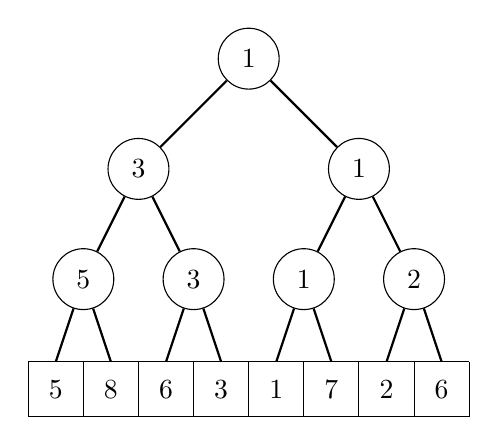
\begin{tikzpicture}[scale=0.7]
\draw (0,0) grid (8,1);

\node[anchor=center] at (0.5, 0.5) {5};
\node[anchor=center] at (1.5, 0.5) {8};
\node[anchor=center] at (2.5, 0.5) {6};
\node[anchor=center] at (3.5, 0.5) {3};
\node[anchor=center] at (4.5, 0.5) {1};
\node[anchor=center] at (5.5, 0.5) {7};
\node[anchor=center] at (6.5, 0.5) {2};
\node[anchor=center] at (7.5, 0.5) {6};

\node[draw, circle,minimum size=22pt] (a) at (1,2.5) {5};
\path[draw,thick,-] (a) -- (0.5,1);
\path[draw,thick,-] (a) -- (1.5,1);
\node[draw, circle,minimum size=22pt] (b) at (3,2.5) {3};
\path[draw,thick,-] (b) -- (2.5,1);
\path[draw,thick,-] (b) -- (3.5,1);
\node[draw, circle,minimum size=22pt] (c) at (5,2.5) {1};
\path[draw,thick,-] (c) -- (4.5,1);
\path[draw,thick,-] (c) -- (5.5,1);
\node[draw, circle,minimum size=22pt] (d) at (7,2.5) {2};
\path[draw,thick,-] (d) -- (6.5,1);
\path[draw,thick,-] (d) -- (7.5,1);

\node[draw, circle,minimum size=22pt] (i) at (2,4.5) {3};
\path[draw,thick,-] (i) -- (a);
\path[draw,thick,-] (i) -- (b);
\node[draw, circle,minimum size=22pt] (j) at (6,4.5) {1};
\path[draw,thick,-] (j) -- (c);
\path[draw,thick,-] (j) -- (d);

\node[draw, circle,minimum size=22pt] (m) at (4,6.5) {1};
\path[draw,thick,-] (m) -- (i);
\path[draw,thick,-] (m) -- (j);
\end{tikzpicture}
\end{center}

U ovom slučaju svaki čvor stabla sadrži
najmanju vrijednost u pripadnom
intervalu niza.
Najviši čvor stabla sadrži najmanju
vrijednost u cijelom nizu.
Operacije se mogu implementirati kao i prije,
samo što se umjesto suma računaju minimumi.

Struktura segmentnog stabla omogućuje nam i
korištenje binarnog traženja za pronalaženje elemenata niza.
Na primjer, ako stablo podržava upite za minimum,
poziciju elementa s najmanjom vrijednosti
možemo pronaći u $O(\log n)$ vremenu.

Na primjer, u gornjem se stablu
element s najmanjom vrijednosti 1 može pronaći
prolaskom putem prema dolje od najvišeg čvora:

\begin{center}
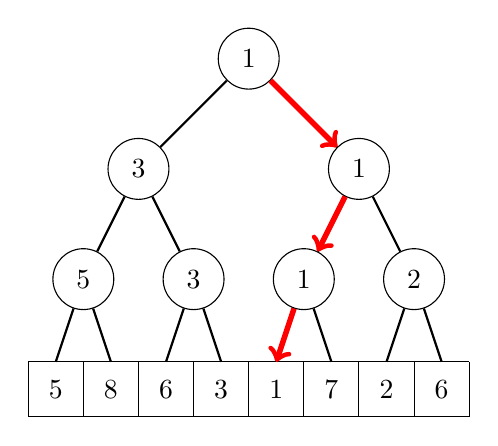
\begin{tikzpicture}[scale=0.7]
\draw (0,0) grid (8,1);

\node[anchor=center] at (0.5, 0.5) {5};
\node[anchor=center] at (1.5, 0.5) {8};
\node[anchor=center] at (2.5, 0.5) {6};
\node[anchor=center] at (3.5, 0.5) {3};
\node[anchor=center] at (4.5, 0.5) {1};
\node[anchor=center] at (5.5, 0.5) {7};
\node[anchor=center] at (6.5, 0.5) {2};
\node[anchor=center] at (7.5, 0.5) {6};

\node[draw, circle,minimum size=22pt] (a) at (1,2.5) {5};
\path[draw,thick,-] (a) -- (0.5,1);
\path[draw,thick,-] (a) -- (1.5,1);
\node[draw, circle,minimum size=22pt] (b) at (3,2.5) {3};
\path[draw,thick,-] (b) -- (2.5,1);
\path[draw,thick,-] (b) -- (3.5,1);
\node[draw, circle,minimum size=22pt] (c) at (5,2.5) {1};
\path[draw,thick,-] (c) -- (4.5,1);
\path[draw,thick,-] (c) -- (5.5,1);
\node[draw, circle,minimum size=22pt] (d) at (7,2.5) {2};
\path[draw,thick,-] (d) -- (6.5,1);
\path[draw,thick,-] (d) -- (7.5,1);

\node[draw, circle,minimum size=22pt] (i) at (2,4.5) {3};
\path[draw,thick,-] (i) -- (a);
\path[draw,thick,-] (i) -- (b);
\node[draw, circle,minimum size=22pt] (j) at (6,4.5) {1};
\path[draw,thick,-] (j) -- (c);
\path[draw,thick,-] (j) -- (d);

\node[draw, circle,minimum size=22pt] (m) at (4,6.5) {1};
\path[draw,thick,-] (m) -- (i);
\path[draw,thick,-] (m) -- (j);

\path[draw=red,thick,->,line width=2pt] (m) -- (j);
\path[draw=red,thick,->,line width=2pt] (j) -- (c);
\path[draw=red,thick,->,line width=2pt] (c) -- (4.5,1);
\end{tikzpicture}
\end{center}

\section{Dodatne tehnike}

\subsubsection{Kompresija indeksa}

Ograničenje struktura podataka
izgrađenih nad nizom jest to
što su elementi indeksirani
uzastopnim cijelim brojevima.
Poteškoće nastaju kada su potrebni
veliki indeksi.
Na primjer, ako želimo koristiti indeks $10^9$,
niz bi morao sadržavati $10^9$
elemenata, što bi tražalo previše memorije.

\index{kompresija indeksa}

Međutim, to ograničenje često možemo zaobići
korištenjem \key{kompresije indeksa},
kod koje se izvorni indeksi zamjenjuju
indeksima $1,2,3,$ itd.
To je moguće učiniti ako unaprijed znamo sve indekse
potrebne tijekom algoritma.

Ideja je svaki izvorni indeks $x$
zamijeniti s $c(x)$, gdje je $c$ funkcija koja
komprimira indekse.
Zahtijevamo da se poredak indeksa
ne mijenja, dakle ako je $a<b$, onda je $c(a)<c(b)$.
To nam omogućuje da udobno izvodimo upite
i kada su indeksi komprimirani.

Na primjer, ako su izvorni indeksi
$555$, $10^9$ i $8$, novi su indeksi:

\[
\begin{array}{lcl}
c(8) & = & 1 \\
c(555) & = & 2 \\
c(10^9) & = & 3 \\
\end{array}
\]

\subsubsection{Ažuriranja nad intervalima}

Do sada smo implementirali strukture podataka
koje podržavaju upite nad intervalima i ažuriranja
pojedinačnih vrijednosti.
Razmotrimo sada suprotnu situaciju,
u kojoj trebamo ažurirati intervale i
dohvaćati pojedinačne vrijednosti.
Usredotočimo se na operaciju koja povećava sve
elemente u intervalu $[a,b]$ za $x$.

\index{niz razlika}

Iznenađujuće, strukture podataka predstavljene
u ovom poglavlju možemo koristiti i u ovoj situaciji.
Da bismo to učinili, gradimo \key{niz razlika}
čije vrijednosti označavaju
razlike između uzastopnih vrijednosti
u izvornom nizu.
Stoga je izvorni niz
niz prefiksnih suma
niza razlika.
Na primjer, promotrimo sljedeći niz:

\begin{center}
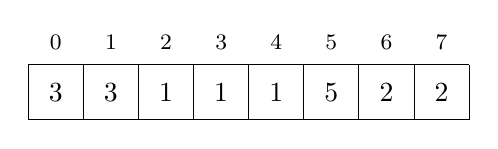
\begin{tikzpicture}[scale=0.7]
\draw (0,0) grid (8,1);

\node at (0.5,0.5) {$3$};
\node at (1.5,0.5) {$3$};
\node at (2.5,0.5) {$1$};
\node at (3.5,0.5) {$1$};
\node at (4.5,0.5) {$1$};
\node at (5.5,0.5) {$5$};
\node at (6.5,0.5) {$2$};
\node at (7.5,0.5) {$2$};


\footnotesize
\node at (0.5,1.4) {$0$};
\node at (1.5,1.4) {$1$};
\node at (2.5,1.4) {$2$};
\node at (3.5,1.4) {$3$};
\node at (4.5,1.4) {$4$};
\node at (5.5,1.4) {$5$};
\node at (6.5,1.4) {$6$};
\node at (7.5,1.4) {$7$};
\end{tikzpicture}
\end{center}

Niz razlika za gornji niz izgleda ovako:
\begin{center}
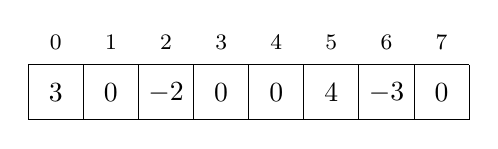
\begin{tikzpicture}[scale=0.7]
\draw (0,0) grid (8,1);

\node at (0.5,0.5) {$3$};
\node at (1.5,0.5) {$0$};
\node at (2.5,0.5) {$-2$};
\node at (3.5,0.5) {$0$};
\node at (4.5,0.5) {$0$};
\node at (5.5,0.5) {$4$};
\node at (6.5,0.5) {$-3$};
\node at (7.5,0.5) {$0$};


\footnotesize
\node at (0.5,1.4) {$0$};
\node at (1.5,1.4) {$1$};
\node at (2.5,1.4) {$2$};
\node at (3.5,1.4) {$3$};
\node at (4.5,1.4) {$4$};
\node at (5.5,1.4) {$5$};
\node at (6.5,1.4) {$6$};
\node at (7.5,1.4) {$7$};
\end{tikzpicture}
\end{center}

Na primjer, vrijednost 2 na poziciji 6 u izvornom nizu
odgovara sumi $3-2+4-3=2$ u nizu razlika.

Prednost je niza razlika u tome
što interval u izvornom nizu
možemo ažurirati mijenjajući samo
dva elementa niza razlika.
Na primjer, ako želimo 
povećati vrijednosti izvornog niza 
između pozicija 1 i 4 za 5,
dovoljno je vrijednost niza razlika
na poziciji 1 povećati za 5
i vrijednost na poziciji 5 smanjiti za 5.
Rezultat izgleda ovako:

\begin{center}
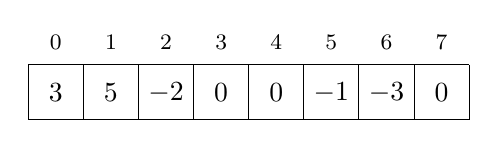
\begin{tikzpicture}[scale=0.7]
\draw (0,0) grid (8,1);

\node at (0.5,0.5) {$3$};
\node at (1.5,0.5) {$5$};
\node at (2.5,0.5) {$-2$};
\node at (3.5,0.5) {$0$};
\node at (4.5,0.5) {$0$};
\node at (5.5,0.5) {$-1$};
\node at (6.5,0.5) {$-3$};
\node at (7.5,0.5) {$0$};

\footnotesize
\node at (0.5,1.4) {$0$};
\node at (1.5,1.4) {$1$};
\node at (2.5,1.4) {$2$};
\node at (3.5,1.4) {$3$};
\node at (4.5,1.4) {$4$};
\node at (5.5,1.4) {$5$};
\node at (6.5,1.4) {$6$};
\node at (7.5,1.4) {$7$};
\end{tikzpicture}
\end{center}

Općenitije, da bismo povećali vrijednosti
u intervalu $[a,b]$ za $x$,
povećavamo vrijednost na poziciji $a$ za $x$
i smanjujemo vrijednost na poziciji $b+1$ za $x$.
Dakle, potrebno je samo ažurirati pojedinačne vrijednosti
i obrađivati upite za sumu,
pa možemo koristiti binarno indeksirano stablo ili segmentno stablo.

Teži je zadatak podržati i
upite nad intervalima i ažuriranja nad intervalima.
U 28. poglavlju vidjet ćemo da je i to moguće.



